
\chapter{Sociální síť Facebook}
\label{chapter:facebook}
    S necelými 2.8 miliardami aktivních uživatelů\footnote{Je myšleno takoví, kteří se přihlásili do sítě alespoň jednou za posledních 30 dní měření. Údaj nezahrnuje Instagram ani WhatsApp.} ke konci čtvrtého čtvrtletí roku 2020 je Facebook největší sociální sítí současnosti~\citep{tankovska_2021}. Se světovou populací okolo 7.8 miliard tvoří jeho uživatelé asi 36 procent světové populace~\citep{unitednations_2019}. 
    
    V České republice je pak toto procento ještě vyšší - aktivních uživatelů Facebooku je 5.6 milionů~\citep{tankovska_2021_a}. Z čehož vyplývá, že v porovnání s počtem obyvatel, kterých bylo k září roku 2020 zaokrouhleně 10.7 milionů, je uživatelů Facebooku přibližně 50 procent obyvatel neboli každý druhý občan~\citep{CSUobyvatele}. 
    
    Takové množství uživatelů se podílí na vzniku enormního množství obsahu, které přispívá k informační přehlcenosti. Jen v roce 2009 Facebook vytvářel 24 \% veškerého sdíleného obsahu na internetu~\citep{carlson_2009}. Informační přehlcenost je tak většinou na Facebooku (stejně jako na jiných platformách) řešena filtrováním dat, které nejsou pro uživatele relevantní - personalizovaným „feedem“. To následně vede k filtračním bublinám o kterých se často mluví ve spojení právě s Facebookem.~\citep{nagulendra2014understanding} 
    
    K pochopení fungování, filosofie a strategie tohoto internetového giganta je však důležitá nejen uživatelská znalost, ale také hlubší pohled do historie a vývoje této společnosti. A protože Facebook hraje centrální roli v této práci, je stěžejní porozumět, jak jeho roli ve společnosti, tak jeho vztahu k filtračním bublinám. 

%%%%% ===============================================================================

\section{Historie a vývoj}
\label{sec:historie-vyvoj}
    Počátek vzniku Facebooku je datován do února roku 2004, kdy jej oficiálně spustil jeho zakladatel Mark Zuckerberg, student Harvardské univerzity, který měl ve svém portfoliu už tehdy několik webových aplikací~\citep{phillips_2007}. Za další zakladatele jsou považováni Eduardo Saverin, Dustin Moskovitz a Chris Hughes~\citep{Hall_2021}. Facebook, který se v té době ještě jmenovala „The Facebook“, byl původně univerzitní sociální sítí, která nejdříve získala svou oblíbenost na Zuckerbergerově alma mater a poté se šířila na další prestižní Ivy League univerzity a nakonec na ostatní univerzity ve Spojených státech a později i na střední školy~\citep{phillips_2007}. 
    
    Už v roce 2004 Facebook do sítě zakomponoval dva důležité prvky, které pro něj dodnes zůstávají charakteristické. „Zeď“ na které mohli uživatelé prezentovat své názory a reklamu, na které dodnes stojí financování společnosti a za kterou platil mezi prvními například MasterCard. S jedním milionem aktivních uživatelů ke konci roku 2004 šlo o rychle rozvíjející se platformu s velkým potenciálem, která „šlapala na paty“ do té doby největší sociální síti MySpace.~\citep{Hall_2021} 
    
    
    Rok poté Facebook přestavil další známé funkce jako například označování přátel. Ke konci roku 2005 měl už 6 milionů aktivních uživatelů (O milion více, než MySpace v předešlém roce).~\citep{Hall_2021}
    
    
    V roce 2005 se Facebooku, svým vstupem mezi Britské univerzity, stal mezinárodní sítí a o rok později bylo přihlášení na platformu umožněno komukoliv s platným e-mailem.~\citep{phillips_2007} V roce 2006 pak byla snížena hranice pro přihlášení na 13 let.~\citep{andrewgreiner_fiegerman_sherman_baker_2019}
    
    Spolu s vývojem nových funkcí a růstem počtu uživatelů přišly také první obavy o soukromí, které od té doby Facebook kontinuálně provází. Konkrétně vznik facebookového „news feedu“ vyvolal u uživatelů vlnu nevole, která vedla k řadě protestů~\citep{andrewgreiner_fiegerman_sherman_baker_2019}. Hlavní problém spočíval v tom, že se na zdi zobrazovala veškerá aktivita, kterou uživatelé na Facebooku uskutečnili. Po několika dalších aplikacích, které podle uživatelů příliš zasahovali do jejich soukromí, se postupně vyvinula nedůvěra k Facebooku a jeho opatřeních k ochraně soukromí. To se také ukázalo v průzkumu z roku 2010, kdy skončil Facebook mezi dolními 5 procenty společností v oblasti zákaznické spokojenosti, a to především kvůli obavám o soukromí.~\citep{Hall_2021}
    
    V roce 2009 uskutečnil Facebook důležitou změnu v doporučování obsahu. Místo „žívého feedu“, který uživatelům zobrazoval aktivity jejich přátel v časové posloupnosti, v jaké se udály, začal obsah řadit na základě jeho údajné kvality. Cílem bylo přinášet uživatelům obsah, který pro ně bude zábavný a relevantní. V podstatě jde o řazení tak jak ho více méně známe dodnes. Na základě řady faktorů - likes, komentáře a pravděpodobnost interakce s obsahem je obsah distribuován na jednotlivé zdi. Facebook se tak posunul k menší transparentnosti.~\citep{bunz_2009} Tahle změna byla možná i díky tomu, že Facebook ve stejném roce zapnul tlačítko liků.~\citep{andrewgreiner_fiegerman_sherman_baker_2019} 
    
    Facebook se postupem řasu stal nejen sociální platformou, která umožňuje propojovat se s přáteli, udržovat s nimi kontakt a sdílet s nimi vzpomínky a zážitky, ale vyvinul se také v platformu s podstatným politickým významem. 
    
    Facebook (spolu s dalšími sociálními sítěmi) hrál důležitou roli v průběhu takzvaného Arabského jara~\citep{Wolfsfeld_andothers}. Konkrétním příkladem je povstání v Egyptě, které odstartoval tehdy 29 letý Wael Ghonim, který na svém Facebooku narazil na fotku k smrti ubitého Khaleda Mohameda Said z Alexandrie místní policií. Událost ho natolik pobouřila, že založil skupinu s názvem „Všichni jsme Khaled Said“.\footnote{Původně „Kullena Khaled Said“ a přeloženo do angličtiny jako „We Are All Khaled Said“.} O tři měsíce později se ke stránce přidalo už více než 250 000 uživatelů. Tato událost nakonec vedla k povstání, které skončilo rezignací prezidenta Hosni Mubaraka a rozpuštění Národní demokratické rady, která byla v té době vládnoucí stranou. Ghonim, který byl během protestů zatčen, se nakonec stal jednou z hlavních tváří Arabského jara.~\citep{vargas_2012}
    
    Z hlediska celkové vlivu Facebooku na veřejné mínění jsou ale důležitější události z roku 2016, které demonstrují význam a sílu Facebooku v současné společnosti, a které zároveň odhalují potenciální hrozby a rizika této platformy (nejen) pro svobodu a demokracii. ~\citep{andrewgreiner_fiegerman_sherman_baker_2019} 
    
    První je zpověď bývalých zaměstnanců Facebooku, zveřejněna na stránce Gizmodo, kteří přiznali, že zaměstnanci Facebooku potlačovali konzervativní zprávy v sekci populárních zpráv. Ta byla zpravována jako v tradiční redakci a podléhala tak subjektivitě a zaujatosti redaktorů.~\citep{nunez_2016} 
    
    Druhou z nich je dosud asi nejvíce diskutována politická událost, která je spojována s Facebookem a to jak v mediích~\citep{lapowsky_2017, madrigal_2017, olson_2016, solon_2016}, tak v akademických kruzích~\citep{Bossetta, Davies, Groshek, Krafft2017, ziegler2018international}. Prezidentské volby, které se odehrály v roce 2016 a jejichž výhercem se stal Donald Trump.~\citep{roberts_siddiqui_jacobs_gambino_holpuch_2016} 
    
    
    \setlength\parskip{5mm}
    
    \textit{„Fake news, boti na sociálních sítích (automatizované účty, které se mohou objevovat na různých druzích platforem) a propaganda uvnitř i vně Spojených států - spolu s revolučními způsoby používání nových médií výherní kampaní - dohromady narušili zavedená paradigmata toho, jak kandidovat na prezidenta.“}\footnote{Přeloženo z: Fake news, social-media bots (automated accounts that can exist on all types of platforms), and propaganda from inside and outside the United States -  alongside revolutionary uses of new media by the winning campaign - combined to upset established paradigms of how to run for president.}~\citep{persily20172016} To vše jsou skutečnosti, které charakterizovaly prezidentské volby v roce 2016. 
    
    Přestože je zásah zahraničních vlád, jednotlivců nebo institucí do voleb ve Spojených státech nelegální, přetrvává obava, že ruská vojenská zpravodajská služba investovala své finanční zdroje do různých sociálních platforem s cílem ovlivnit výsledky právě těchto voleb. V letech 2015 a 2017 bylo na Facebooku (cíleno na US, ne celkově) zakoupeno přibližně 3500 reklam v ruských rublech. Tyto reklamy byly předpojaté vůči demokratům oproti republikánům a jejich povaha naznačuje snahu rozdělit společnost (v politických, rasový a náboženských ideologiích).~\citep{dutt2018senator} 
    
    \setlength\parskip{0mm}
    
    Tento nový způsob využívání reklamy na sítích s cílem vyvolání sociálního konfliktu nazývá~\cite{ribeiro2019microtargeting} jako „sociálně rozdělující reklama“. A dále také potvrzuje, že facebooková reklama může být zneužívaná tímto způsobem. Ruské reklamy spojované s prezidentskou kampaní v roce 2016 se ukázaly jako pro společnosti rozdělující a navíc jako desetkrát účinnější než běžná facebooková reklama. Tyto příspěvky byly rasově i politicky předpojaté a byly cíleny na skupinu uživatelů, která má nižší potenciál rozeznat povahu těchto reklam. Kromě facebookových reklam tito inzerenti ke svým cílům zneužívali také facebookový doporučovací algoritmus k organizování cílového publika.
    
    Odhlédneme-li k výsledkům těchto studií, které byli publikovány až pár let po volbách, Mark Zuckerberg bezprostředně po volbách popřel možnost, že by výsledky voleb mohli být ovlivněny fake news a jakoukoliv jinou manipulací třetích stan. \textit{„Osobně si myslím, že představa, že fake news na Facebooku, kterých je v celkovém obsahu velmi malé množství, by jakýmkoliv způsobem ovlivnily volby, je docela šílená představa.“}\footnote{Přeloženo z: “Personally, I think the idea that fake news on Facebook, of which it’s a very small amount of the content, influenced the election in any way is a pretty crazy idea,” Zuckerberg said.} Zároveň přiznal, že problémem mohl být interakce (příspěvky podporující Donalda Trumpa jich obdrželi více, proto byl i lepší předpoklad k jejich šíření) a neprůhlednost facebookové algoritmu - potenciál pro vznik filtračních bublin. Ve své reakci také projevil důvěru ve schopnosti uživatelů rozeznat nepravdivý obsah.~\citep{mannes_2016}
    
    V roce 2018 Facebook navázal další kauzou spojenou se společností Cambridge Analitica, která spolupracovala v roce 2016 s Donaldem Trumpem na jeho prezidentské kampani~\citep{andrewgreiner_fiegerman_sherman_baker_2019} a pracovala také na vítězné Brexit kampani~\citep{cadwalladr_graham-harrison_2018}. To se stalo podnětem pro výslech Marka Zuckerbega, CEO Facebooku, v kongresu, kde se musel zpovídat z toho, jak společnost nakládá s daty a jak chrání soukromí svých uživatelů~\citep{andrewgreiner_fiegerman_sherman_baker_2019}.
    
    Společnost v roce 2014 využila neautorizovaná data uživatelů Facebooku, která následně použila k sestavení jejich profilu a lepšímu cílení. Skrze aplikaci „tohlejetvůjdigitálníživot“\footnote{V originále: thisisyourdigitallife} sesbírali nejen data stovek tisíc uživatelů, kteří udělili souhlas s použitím dat, ale také jejich přátel, čímž získali miliony uživatelských dat. Facebook udělil povolení pouze sbírat data za účelem zlepšení uživatelské zkušenosti aplikace a zakazoval jejich využití pro komerční účely~\citep{cadwalladr_graham-harrison_2018}. 
    
    Tento neoprávněný sběr důvěrných informací o uživatelích byl možný hned z několik důvodů. Asi ten nejdůležitější je nedostatečná ochrana a vytyčení hranic vůči organizacím, které se zabývají sběrem dat. Dále pochybení na straně vývojářů Facebooku (neadekvátní dohled nad daty) a nakonec nadměrné schvalování podmínek a pravidel na Facebooku na straně uživatelů.~\citep{ur2019facebook}
    
    \setlength\parskip{5mm}
    
    \textit{„Cambridge Analytica skandál odstartoval největší krizi publicity, kterou Facebook dosud zažil. Způsobil nahromadění strachu, že algoritmus, který determinuje, co lidé na platformě vidí, množí fake news a nenávistné projevy, a že je ruští hackeři využili jako zbraň ve snaze ovlivnit volby v Trumpův prospěch. Miliony si začaly mazat aplikaci; zaměstnanci na protest dali výpověď; kapitalizace firmy na trhu se propadla o více než 100 billionů dolarů po červencové finančním reportování.“}\footnote{Přeloženo z originálu: The Cambridge Analytica scandal would kick off Facebook’s largest publicity crisis ever. It compounded fears that the algorithms that determine what people see on the platform were amplifying fake news and hate speech, and that Russian hackers had weaponized them to try to sway the election in Trump’s favor. Millions began deleting the app; employees left in protest; the company’s market capitalization plunged by more than \$ 100 billion after its July earnings call.}~\citep{hao_2021}
    
    Kauza Facebook a Cambridge Analytica je novým milníkem v historii internetu a jen dále ilustruje, že nastavení regulujících pravidel ve Facebooku zaostává za technologickým vývojem, který může být bez regulace ohrožující pro demokratickou společnost. Jen soubor preventivních pravidel a edukace veřejnosti mohou zvrátit současný trend zvyšujícího se technologického elitářství a úpadku soukromí.~\citep{common2018facebook}
    
    Všechny výše popsané události utvářely Facebook, jak jej známe v současnosti. Filosofie společnosti a její hodnoty dávají vzniknout jednotlivým funkcím a algoritmům, které se následně mohou podílet na vzniku filtračních bublin. Jak se společnost vyvíjela může být podstatným ukazatelem toho, jak bude postupovat v budoucnu, což může být důležitou perspektivou pro řešení problému filtračních bublin. Proč je engagement důležitým činitelem ve vzniku filtračních bublin a jak k jejich potlačení v současnosti Facebook přistupuje, popisuje následující podkapitola.
    
    \setlength\parskip{0mm}
%%%%% ===============================================================================
\section{Doporučovací algoritmus - za vším hledej engagement}
\label{sec:doporucovaci-algoritmus-engagement}
 
    Zuckerberg na kauzu Cambridge Analytica reagoval příslibem, že Facebook změní svou politiku a stane se z něj platforma, která je postavena na základech soukromí a ochrany uživatelských dat.~\citep{shaban_2019} Facebook slibuje nejen, že udělá ze soukromí a bezpečnosti svých uživatelů svoji prioritu, ale také že se pokusí být mnohem transparentnější a bude se snažit, aby jeho uživatelé získali lepší pochopení facebookového algoritmu - proč na svých zdech vidí to, co vidí.~\citep{satterfield_2020} Mimo jiné by mělo být podle Zuckerberga aplikováno šest základních principů: soukromí během interakcí, šifrování, méně trvalý obsah, bezpečnost, propojení s dalšími aplikacemi Facebooku, bezpečné uložiště dat.~\citep{zuckerberg_2021} Facebook však (alespoň donedávna) vždy prioritizoval svůj vlastní růst nad soukromým svých uživatelů. Proto zůstává otázkou, zda je schopný dostát svým slibům.~\citep{lapowsky_2019}
    
    Přestože byl ve Facebooku sestaven speciální tým, který má zjednodušeně na starosti zodpovědnější algoritmus, snahy o implementaci etických zásad za pomocí pravidel definovaných v nástroji „Fairness Flow“ pro vývojáře (který tento tým vyvinul), nejsou zatím ze strany Facebooku vynucovány. Některé části kódu, které by mohly předcházet negativním efektům facebookové AI, jsou dokonce cíleně odmítnuty. Důvodem je dosavadní nastavení společnosti, které charakterizuje slovo „růst“ a na níž je navázáno také ohodnocení vývojářů. 
    
    
    Růst sám o sobě má pro Facebook velmi jasné a charakteristické hranice, které jsou definovány takzvaným „engagementem“\footnote{Českým ekvivalentem by bylo slovo „interakce“.}. Tato metrika je v podstatě určující pro růst společnosti a jsou ji podřízeny veškeré aktivity společnosti.~\citep{hao_2021}
    
    \setlength\parskip{5mm}
    
    \textit{„V roce 2017 Chris Cox, dlouholetý hlavní produktový manažer Facebooku, vytvořil nový tým, aby porozuměl tomu, zda maximalizace engagementu na Facebooku přispívá politické polarizaci. Zjistil, že zde skutečně existuje korelace a že snížení polarizace by znamenalo ránu pro enagagement. V dokumentu z poloviny roku 2018, který byl revidovaný the Journal, tato pracovní skupina navrhla několik potenciálních řešení jako vyladění doporučovacího algoritmu tak, aby navrhoval různorodější spektrum skupin, ke kterým se lidé pomohou přidat. Dokument přiznával, že některé nápady byly „proti růstu“. Většina těchto návrhů neprošla a pracovní skupina se rozpadla.“}\footnote{In 2017, Chris Cox, Facebook’s longtime chief product officer, formed a new task force to understand whether maximizing user engagement on Facebook was contributing to political polarization. It found that there was indeed a correlation, and that reducing polarization would mean taking a hit on engagement. In a mid-2018 document reviewed by the Journal, the task force proposed several potential fixes, such as tweaking the recommendation algorithms to suggest a more diverse range of groups for people to join. But it acknowledged that some of the ideas were “antigrowth.” Most of the proposals didn’t move forward, and the task force disbanded.}
    
    Jinými slovy se ukázalo, že čím více porušují příspěvky Facobookové zásady komunity, tím více pozornosti a engagementu obdrží od uživatelů - algoritmus, jehož cílem je maximalizace engagementu, tak logicky odmění nenávistný obsah lepším dosahem (jak je ukázáno na obrázku~\ref{fig:fb-enagement}). Tedy ve snaze nabídnout uživateli další relevantní obsah mu potenciálně může nabídnout další dezinformaci. Řešení tohoto problému je vyvinutí nové AI, která by tento obsah rozpoznávala a cíleně by jeho dosah zpětně snižovala - AI se nejdříve potřebuje naučit obsah rozeznat a následně trvá jeho identifikace, po kterou se může obsah ještě šířit. Tento způsob však není neprůstřelný a uživatelé se mohou naučit obcházet algoritmus například eufemismy, sarkasmem atd.~\citep{hao_2021}
    \setlength\parskip{0mm}
    
    \begin{figure}[H]
        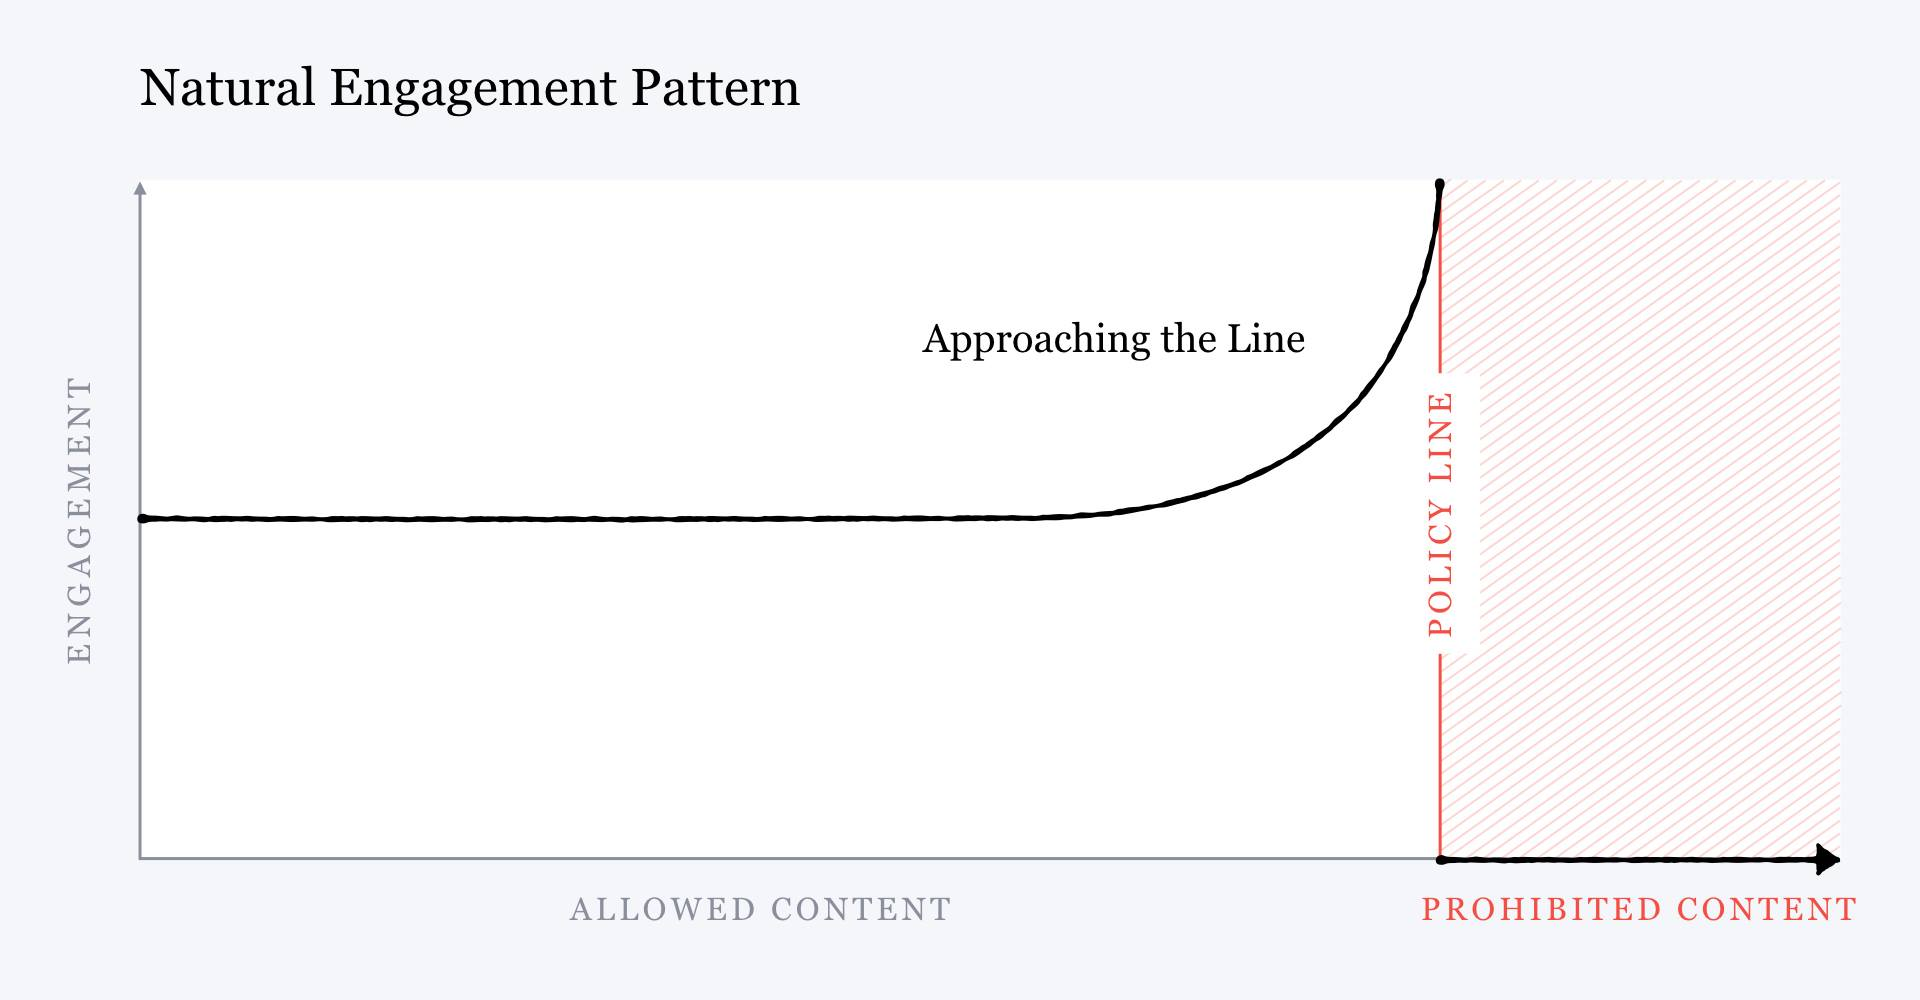
\includegraphics[width=\linewidth]{obrazky/fb_engagement.jpeg}
        \centering
        \label{fig:fb-enagement}
        \caption[Facebook Engagement]{Facebook Engagement. Zdroj: https://bit.ly/TRFBmisinformation}
    \end{figure}
    
    Aktuální studii, která se zaměřovala na volby v roce 2020, uskutečnili~\cite{edelson_nguyen_goldstein_goga_lauinger_mccoy_2021}, kteří došli k velmi podobným výsledkům jako výzkumné týmy Facebooku - politicky extrémní příspěvky mají tendeci generovat více uživatelských interakcí. Analýza se zaměřovala na interakci uživatelů s různými typy příspěvků, které vypadaly jako zpravodajství. 
    
    Monica Lee, výzkumnice a socioložka z Facebooku, v roce 2016 uvedla, že na Facebooku se nachází nejen velké množství extrémistických skupin, ale Facebook je navíc propaguje mezi svými uživateli. Až 64 \% uživatelů, kteří se přidali k těmto skupinám, tak učinili na základě doporučovacího systémů - výzvy typu „skupiny, které by se vám mohly líbit“ nebo „objevujte“. Během prezentace na mezinárodní bezpečnostní konferenci v Mnichově vedení společnosti prohlásilo, že se pokusí nedoporučovat skupiny, které jsou polarizující nebo porušují facebooková pravidla.~\citep{horwitz_seetharaman_2020} Problém doporučování extrémistických skupin tak podle všeho nebyl vyřešen ani v roce 2016, ani v roce 2018, kdy se jim zabývala pracovní skupina Chrise Coxe. 
    
    Zuckerberg i nadále přiznává, že Facebook může společnost rozdělovat a že je potřeba určitá míra regulace.~\citep{marson_2020} Na druhou stranu Facebook dosud prioritizoval svůj vlastní růst nad zájmy veřejnosti, a tak je řešení problémů zatím jen tak důležité, jak Facebook sám uzná za vhodné.~\citep{hao_2021}.

%%%%% ===============================================================================

\section{Doporučovací algoritmus - jak to funguje}
\label{chapter:doporucovaci-algoritmus-fungovani}
    Pochopit, jak doporučovací algoritmus Facebooku funguje je důležité nejen pro kontext výzkumu, který byl realizován v rámci této práce, ale také pro porozumění tomu, jaké máme možnosti v ohledu prevence a předcházení vzniku filtračních bublin.
    
    V první řadě stojí za facebookovým algoritmem sofistikovaný kód na bázi strojového učení~\citep{lada_wang_yan_2021}. Každá akce, která je na stránce uskutečněna, ať už komentář nebo like stránky, je využita k personalizaci uživatelské zkušenosti. ~\citep{satterfield_2020} 
    
    Příspěvky, které budou zobrazeny ve facebookovém „feedu“ určitého jedince jsou filtrovány několika stupňovým procesem za pomocí mnoha vrstev strojového učení. Cílem je zobrazovat takový obsah, který bude pro daného člověka relevantní, zajímavý a bude mu přinášet dlouhodobou hodnotu. To je určováno na základě řady faktorů jako: koho nebo co jsme nedávno začali sledovat, co jsme likovali nebo s čím jsme nedávno interagovali, co zajímá naše přátele\dots
    
    Facebooku především usiluje o to, aby uivatelům přinášel smysluplný obsah a vytvářel takzvané smysluplné interakce\footnote{V angličtině jako meaningful interactions.~\citep{facebook_2018} Jedná se o obecný koncept budování komunit, který se vyznačuje pozitivním vlivem na skupiny, ale i jednotlivce.~\citep{department2009guidance} }
    
    Obsahu, který je pro daného jedince relevantní mohou být stovky a tisíce, proto je nejdříve potřeba výběr zúžit a v konečném důsledku determinovat ty nejvýše postavené příspěvky. Na základě toho je vytvořeno několik samostatných modelů současně, které ohodnotí, co by se danému člověku mohlo nejvíce líbit - mohou být protichůdné a nesouhlasit spolu. Pro všechny je však ideálním cílem, aby daný jedinec provedl s doporučeným příspěvkem nějakou akci (engagement).
    
    Potom, co algoritmus každý příspěvek ohodnotí a přidá mu určité skóre, ověří integritu příspěvků - aby se mohly z výběru odfiltrovat fake news a „clickbait“ příspěvky - zúží výběr příspěvků na zhruba 500. Následně je znovu ohodnotí a seřadí podle skóre. Způsob tohoto hodnocení se pro každého může lišit - lidé s příspěvky různě interagují - někteří více likují, jiní zase sdílejí nebo komentují. Nakonec je provedena kontextuální kontrola, která zaručuje, že se ve „feedu“ zobrazí obsah různorodého charakteru (foto, videa, příspěvky, články\dots).~\citep{lada_wang_yan_2021}
    
    Ve zkratce by se celé hodnocení dalo rozvrhnout podle ~\citep{mosseri_2019}, do čtyř základních elementů: 
    \begin{enumerate}
      \item Dostupný \textbf{inventář} příběhů (příspěvků). 
      \item \textbf{Signály}, které jsou informačním základem pro hodnocení.
      \item \textbf{Předpověď} toho, jak se bude obsah líbit uživateli.
      \item \textbf{Skóre relevance} pro každý příběh.
    \end{enumerate} 
    
    Co se týče konkrétně fungování algoritmu, který vybírá stránky, které se zobrazí jako doporučené při zalikování jiné stránky, nelze s jistotou přesně říci, na jakých principech je postavený. Facebook na jednom ze svých webů jasně uvádí, že doporučuje stránky, skupiny a události na základě zájmů a akcí jednotlivých uživatelů tak, aby každý z nich dostával personalizovaná doporučení, která odpovídají jeho zájmům. Aby Facebook „ochránil“ uživatele od obsahu, který pro něj může být potenciálně nebezpečný nebo nevhodný, stanovuje si řadu pravidel pro doporučování obsahu.~\citep{rosen_2020}
    
    Za takový obsah může být považován obsah nízké kvality, nevhodný, obzvláště citlivý nebo nevhodný pro mladé publikum. Konkrétně existuje pět různých kategorií nežádoucího obsahu~\citep{facebook_2021B}:
    \begin{enumerate}
      \item Obsah, který brání podpoře bezpečné komunity (např. násilí, téma sebevraždy nebo poruch příjmu potravy, obsah sdílený nepodporovanou skupinou, obsah promující regulovaný produkt atd.).
      \item Citlivý obsah nebo obsah nízké kvality s tématem zdraví nebo financí (např. obsah, který zobrazuje kosmetické procedury; promování zavádějících business modelů atd. ). 
      \item Obsah, který uživatelů nemají rádi (např. „clickbait“ atd.).
      \item Obsah, který má nízkou kvalitu publikování (např. zprávy, které obsahují netransparentní informace o autorovi nebo vydavateli atd.)
      \item Nepravdivý nebo zavádějící obsah. (např. obsah, který byl shledán jako nepravdivý nezávislými lidmi/institucemi, které ověřují informace atd.) 
    \end{enumerate}
    
    \setlength\parskip{5mm}
    
    Facebook uvedl, že do ledna 2021 už deaktivoval tisíce skupin, které porušovaly jeho zásady komunity a šířily nepravdivý nebo nenávistný obsah. Proti stránkám, které (zatím) tvrdě neporušují pravidla Facebooku, ale jejich obsah může být potenciálně nebezpečný, se sociální síť rozhodla, mimo jiné, zasáhnout následujícími způsoby. Cílem je omezit formování těchto skupin na platformě~\citep{facebook_2021A}.
    \setlength\parskip{0mm}
    \begin{itemize}
        \item \textbf{Odstranění z Facebooku:} Neprodleně po tom, co se na stránkách objeví nepravdivý nebo nenávistný obsah.
        \item \textbf{Omezení doporučení:} Stránky nebudou doporučeny mezi podobnými stránkami. 
        \item \textbf{Zhoršit kvalitu vyhledávání:} Stránky nebude snadné na platformě dohledat.
        \item \textbf{Odstranění z Facebooku:} Neprodleně po tom, co se na stránkách objeví nepravdivý nebo nenávistný obsah.
    \end{itemize}

%%%%% ===============================================================================















%%%%% ===============================================================================

%%%\begin{table}[b!]

%%\centering
%%% The following packages are needed for this example:
%%%   - booktabs (\toprule, \midrule, \bottomrule)
%%%   - dcolumn (column type  D)
%%% Commands \pulrad and \mc defined in BcPrace.tex are used

%%%\begin{tabular}{l@{\hspace{1.5cm}}D{.}{.}{3.2}D{.}{.}{1.2}D{.}{.}{2.3}}
%%%\toprule
%%% & \mc{} & \mc{\textbf{Std.}} & \mc{} \\
%%% \pulrad{\textbf{Effect}} & \mc{\pulrad{\textbf{Estimate}}} & \mc{\textbf{error}$^a$} & 
%%% \mc{\pulrad{\textbf{P-value}}} \\
%%%\midrule
%%%Intercept     & -10.01 & 1.01 & \mc{---} \\
%%%Gender (male) & 9.89   & 5.98 & 0.098 \\
%%%Height (cm)    & 0.78   & 0.12 & <0.001 \\ 
%%%\bottomrule
%%%\multicolumn{4}{l}{\footnotesize \textit{Note:} 
%%%$^a$ Standard error of the estimator by the Monte Carlo method.}
%%%\end{tabular}%%%

%\caption{Maximum likelihood estimates from model M.}\label{tab03:Nejaka}

%%%\end{table}


%%%\textbf{Tables} should be formatted according to the following rules:
%%%\begin{compactitem} %% requires package paralist
%%%\item Avoid vertical lines. Separate the table from the surrounding
%%% text (even the legend) by stronger horizontal lines. Separate the
%%% header from the table and different parts of the table from each
 %%% other by thinner horizontal lines. This table format can be obtained
 %%% in \LaTeX\ by loading the package \texttt{booktabs}. If a stronger
 %%% separation of the columns is desired it can be achieved by including
 %%% an additional vertical space. 
%%%\item Do not change the type, format and meaning of the cells in a
%%%  single column (never include means in some cells and percentages in
%%%  other cells of the same column).
%%%\item Do not repeat the same cell contents many times. If the table
 %%% includes the column ``Variance'', which contains the value 0.5 in
  %%%the first ten cells and 1.5 in the next ten cells, delete this
 %%% column and find another way to communicate the value of the
 %%% variance. For example, the table can be divided into two separate
 %%% tables and the variance given in the legend. Or additional rows can
%%%  be included between the parts of the table informing what was the
%%%  variance in the subsequent rows.
%%%\item Numeric columns in the table should be aligned on the decimal
%%%  point. 
%%%\item Tables sometimes include abbreviations that are not used
%%%  elsewhere in the text. These abbreviations should be explained i%%% the legend or in notes under the table. These notes can be also used
 %%% to provide more detail on the meaning of selected columns or cells. 
%%%\end{compactitem}




%%%\section{Figures}

%%%Some advice on figures and diagrams:
%%%\begin{compactitem}
%%%\item Create the figure in the same size that will be used in the
%%%  thesis. Excessive magnification or reduction of figures causes poor
%%%  readability.
%%%\item The axes of a graph must be carefully annotated in the same
%%%  language the thesis is written in. Units of measurement (kg,
%%%  minutes, \ldots) should be provided when applicable. When the graph
%%%  plots a function $h(x)$ the axes should be annotated by $x$ a
%%%  $h(x)$. Each axis must have a clearly defined scale (tickmarks, labels).
%%%\item If a two-dimensional scatterplot includes a large number of
%%%  points make sure that the points do not turn into black cloud. If
%%%  the number of points is too large reduce the size of the plotting
%%%  symbol or select a subset of the points. Plots that include
%%%  thousands of points make problems in electronic documents, they
 %%% increase the size too much.
%%%\item If the thesis is to be printed on a black-and-white printer, do
%%%  not use colors. Lines can be distinguished by the type (solid,
 %%% dotted, \ldots), areas can be filled by various shades of grey or 

%%%The meaning of the line types and area shading should be explained in
%%%the legend or directly in the plot.
%%%\end{compactitem}




